
\documentclass[a4paper, twoside]{article}      % Comments after  % are ignored
\usepackage{amsmath,amssymb,amsfonts} % Typical maths resource packages
\usepackage{graphics}                 % Packages to allow inclusion of graphics
\usepackage{color}                    % For creating coloured text and background
\usepackage{hyperref}                 % For creating hyperlinks in cross references

\oddsidemargin 0cm
\evensidemargin 0cm

\pagestyle{myheadings}         % Option to put page headers
                               % Needed \documentclass[a4paper,twoside]{article}

%\markboth{{\small\it PDF\ \LaTeX \ coloured text and graphics}}

%{{\small\it C.T.J. Dodson} }
\textwidth 15.5cm
\topmargin -1cm
\parindent 0cm
\textheight 24cm
\parskip 1mm

\newtheorem{theorem}{Theorem}[section]
\newtheorem{proposition}[theorem]{Proposition}
\newtheorem{corollary}[theorem]{Corollary}
\newtheorem{lemma}[theorem]{Lemma}
\newtheorem{remark}[theorem]{Remark}
\newtheorem{definition}[theorem]{Definition}



\def\R{\mathbb{ R}}

\def\S{\mathbb{ S}}



\date{\small\it April 20, 2009}

\title{\fcolorbox{white}{white}{\color{black}Power / Delay Estimation of Auto Generated Circuits}}

%\footnote{A demonstration example including colored text and graphics}}}



\author{ K. P. Ghosh, S.Subramanian \\
{\small Department of Electrical Engineering, IIT, Bombay, India}
 }










\begin{document}
\maketitle
\begin{abstract}
{
The goal of the research project was to characterize RTL generated by AHIR flow. We had taken a set of examples, used AHIR to generate RTL, mapped the RTL tolayout, and finally performed power, area and delay estimation for the above examples.  For all our circuit examples we have used  OSU Standard Cell library for TSMC 0.18 technology and Synopsis  Design Compiler to perform synthesis. The netlist thus obtained is used as an input to Cadence SOC Encounter  to generate the layout. The layout being closest to the actual hardware is most suiatble for estimation of power consumed in the design for a particular input sequence.Hence, we present an alternate approach of implementing memory in our circuits as Blackboxes. Cacti 3.2[1] was used to model the power and delay of the memory blackboxes. Five examples viz. A5, AES, Red Black trees, Linpack and FFT were selected, six memory architectures were explored for each and results are summarized in final section.
}
\end{abstract}

%{\color{black}{\sc keywords: AHIR, Memory Modelling, Cacti}}

\section{Introduction}
{AHIR provides a platform to describe hardware in a high level programming language like C and translates it to its equivalent hardware description. When we use this description of hardware, followed by the RTL synthesis and then its layout, we would like to characterise the hardware thus generated to meet certain physical and performance criteria. Area , power and delay are  important criteria that mark the quality of the hardware. The current approach followed by us to obtain layout from a VHDL description is as shown in the figure 1. Memories in the hardware have been treated as blackboxes with suitable power and area models obtained from Cacti 3.2.  

\begin{figure}[ht]
{\centering \resizebox*{6in}{4in}{\includegraphics{list_of_figures1.ps}} \par}
\caption{Flow describing VHDL Description to Layout}
\end{figure}

At each level, a different tool is used for a specific purpose. At first,  the VHDL code  is simulated and checked for  its functionality using ModelSim 6.3a. The next step is  to perform synthesis and obtain a gate level netlist. For all our circuit examples we have used  OSU Standard Cell library for TSMC 0.18 technology and Synopsis  Design Compiler (DC) to perform synthesis. The netlist thus obtained is used as an input to Cadence SOC Encounter  to generate the layout. The layout being closest to the actual hardware is most suitable for estimation of powert consumed in the design for a particular input sequence.  Power has been calculated using Cadence SOC Encounter.

The memory could either be built up as a single bank or as a combination of multiple banks. The later would aid parallelism in the circuit. Also, the memory could be pipelined. We have tried to explore 6 different memory architectures for different examples. This would help us compare the performance of the circuits with multiple banks versus single banks, pipelined as opposed to non-pipelined memory. 
}
\section{Memory Modelling}
For encounter to estimate power, delay and area of the entire hardware, the memory black boxes must have the respective information. We use Cacti 3.2 to estimate power and delay in the memory black box. The area is modelled using  [2].

area(in mm2) = (0.001){ * }(tech)^{2.07} { * } (bits)^{0.9} { * } (port)^{0.7} + {0.0048}

The values of power, area and delay obtained from the above models are used to generate the necessary information for the blackboxes in timing library file (TLF) and library exchange file (LEF) formats.The vital timing information is also obtained from delay models. 
To describe a memory element as a black box, we instruct Synopsys DC to turn off its synthesis when it encounters the architecture for the memory.
Thus for synopsys, the memory is an entity definition with well defined input & output ports but a blank architecture.
Similarly, Cadence SOC encounter is made to infer black boxes whenever a memory component is instantiated from the TLF and LEF files.

\section{Power Estimation}
Using the final gate level verilog netlist provided by encounter we perform a post -layout simulation and dump all the signal information to a vcd file. This vcd file which now contains all the switching activity information is used by SOC Encounter to generate a power report. One is also required to mention the top level entity name for which power is to be estimated.
For examples like linpack, Redblack which required huge size of memories and also which took a long time to simulate, a sampling technique was followed, in order to reduce the size of VCD files (which was around 25Gb). In this technique, the final post layout netlist is simulated and the switching activities are captured at 10 random intervals of time. It was observed that, when power is calculated using these samples, the variance in power estimates for all the samples is in the orders of 1e-5.  

\section{Results}
Five examples viz. A5, AES, Red Black trees, Linpack and FFT were selected. 
The memory architecture choices are shown table 1:


\begin{table}[t]

\caption{Architecture choices for each example}
\begin{center}
{\begin{tabular}{c  c | c  c  c}
\hline
ARCHITECTURE && \multicolumn{3}{c}{MEMORY BANK CHOICE} \\  
CHOICES && 1& 2& 4 \\ [3ex] 
\hline
Example& Memory Size &&Base Bank Address Width \\ [1ex]
\hline 
A5& 16& 4& 4& 4\\[1ex]
LINPACK& 16K& 12& 12& 12\\[1ex]
R-B TREES& 16k& 12& 12& 12\\[1ex]
FFT& 512& 8& 8& 8\\[1ex]
AES& 1024& 8& 8& 8\\[1ex]
\hline

\end{tabular}}
\label{diffstruc}
\end{center}	
\end{table}

For each of memory architecture choices, mux and demux degree of 2 and infinity was selected.
The range of frequencies tried for each architecture is shown in table 2:


\begin{table}[t]
\caption{Range of Frequencies for Each Architecture}
\begin{center}
{\begin{tabular}{c | c  c  c  c  c  c}
\hline
 & \multicolumn{6}{c}{ARCHITECTURE CHOICES} \\[1ex]
 &1x2 &1x0 &2x0 &2x2 &4x2 &4x0 \\ [1ex]
\hline
Example& \multicolumn{6}{c}{Frequency of Operation (in MHz)} \\ [1ex]
\hline
A5& 71.42& 71.42& 83.33& 71.42& 83.33& 71.43\\[1ex]
LINPACK& 45.45& 41.67& 41.67& 41.67& 41.67& 38.4\\[1ex]
R-B TREES& 41.67 and 62.5 & 41.67 and 55.56& 71.42& 50& 71.42& 38.36\\[1ex]
FFT& 41.66& 41.66& 41.66& 45.45& 45.45& 45.45\\[1ex]
AES& 45.45 and 71.42& 45.45 and 71.42& 71.42& 71.42& 71.42& 45.45\\[1ex]
\hline

\end{tabular}}
\\[1ex]
Note : Architecture choices are in the form [memory bank x mux/demux degree]. For eg. 4 x 2 indicates an architecture with number of memory banks as 4 and mux/demux degree of 2. 0 indicates a mux/demux degree of infinity.
\label{diffstruc}
\end{center}
\end{table}

\subsection{Reports}
The energy, delay and area estimates for each example with their respective 6 architectures are as follows:

\subsubsection{A5/1}
\\
The energy, delay and area estimates for each architecture / frequency combination is given in table 3.
Figure 2 and 3 shows the Power-Delay and Area-Delay plot for A5/1. 
\begin{table}[h!]
\caption{Energy / Delay / Area for each architecture/frequency combination}
\begin{center}
{\begin{tabular}{|c | c |  c |  c  | c  |  c |  c|}
\hline
A5/1 &1x2 &1x0 &2x0 &2x2 &4x2 &4x0 \\ [1ex]
\hline
Energy &&&&&& \\ [1ex]
\hline
Delay (ns)& 308& 280& 252& 266& 240& 252\\[1ex] \hline
Area (mm^2)& 1.45& 1.3& 1.77& 1.52& 2.3& 1.9\\[1ex]
\hline

\end{tabular}}
\label{diffstruc}
\end{center}
\end{table}


\begin{figure}[h!]
{\centering \resizebox*{6in}{4in}{\includegraphics{a5p.ps}} \par}
\caption{Power-Delay plot for A5/1}
\end{figure}

\begin{figure}[h!]
{\centering \resizebox*{6in}{4in}{\includegraphics{a5a.ps}} \par}
\caption{Area-Delay plot for A5/1}
\end{figure}


\subsubsection{LINPACK}
\\
The energy, delay and area estimates for each architecture / frequency combination is given in table 4.
Figure 4 and 5 shows the Power-Delay and Area-Delay plot for Linpack.

\begin{table}[h!]
\caption{Energy / Delay / Area for each architecture/frequency combination}
\begin{center}
{\begin{tabular}{|c | c |  c |  c  | c  |  c |  c|}
\hline
LINPACK &1x2 &1x0 &2x0 &2x2 &4x2 &4x0 \\ [1ex]
\hline
Energy &&&&&& \\ [1ex]
\hline
Delay (ms)& 56.48& 43.65& 55.63& 37.68& 51.64& 38.71\\[1ex] \hline
Area (mm^2)& 27.5& 25.5& 30.8& 27& 36.2& 28.9\\[1ex]
\hline

\end{tabular}}
\label{diffstruc}
\end{center}
\end{table}


\begin{figure}[h!]
{\centering \resizebox*{6in}{4in}{\includegraphics{lpp.ps}} \par}
\caption{Power-Delay plot for LINPACK}
\end{figure}

\begin{figure}[h!]
{\centering \resizebox*{6in}{4in}{\includegraphics{lpa.ps}} \par}
\caption{Area-Delay plot for LINPACK}
\end{figure}


\subsubsection{R-B TREES}
\\
The energy, delay and area estimates for each architecture / frequency combination is given in table 5.
Figure 6 and 7 shows the Power-Delay and Area-Delay plot for Red-Black Trees.

\begin{table}[h!]
\caption{Energy / Delay / Area for each architecture/frequency combination}
\begin{center}
{\begin{tabular}{|c | c |  c |  c  | c  |  c |  c|}
\hline
R-B TREES &1x2 &1x0 &2x0 &2x2 &4x2 &4x0 \\ [1ex]
\hline
Energy &&&&&& \\ [1ex]
\hline
Delay (ms)& 18.74 and 12.5& 9.88 and 7.41& 10.9& 8.17& 10.87& 10.57\\[1ex] \hline
Area (mm^2)& 19 and 23& 18 and 21& 26& 22& 32& 25\\[1ex]
\hline

\end{tabular}}
\label{diffstruc}
\end{center}
\end{table}


\begin{figure}[h!]
{\centering \resizebox*{6in}{4in}{\includegraphics{rbp.ps}} \par}
\caption{Power-Delay plot for RED-BLACK TREES}
\end{figure}

\begin{figure}[h!]
{\centering \resizebox*{6in}{4in}{\includegraphics{rba.ps}} \par}
\caption{Area-Delay plot for RED-BLACK TREES}
\end{figure}



\subsubsection{FFT}
\\
The energy, delay and area estimates for each architecture / frequency combination is given in table 6.
Figure 8 and 9 shows the Power-Delay and Area-Delay plot for FFT.

\begin{table}[h!]
\caption{Energy / Delay / Area for each architecture/frequency combination}
\begin{center}
{\begin{tabular}{|c | c |  c |  c  | c  |  c |  c|}
\hline
FFT &1x2 &1x0 &2x0 &2x2 &4x2 &4x0 \\ [1ex]
\hline
Energy &&&&&& \\ [1ex]
\hline
Delay (us)& 203.792& 154.88& 189.27& 141.606& 172.453& 140.55\\[1ex] \hline
Area (mm^2)& 5.4& 5.07 & 6.6& 5.7& 9.2& 6.7\\[1ex]
\hline

\end{tabular}}
\label{diffstruc}
\end{center}
\end{table}


\begin{figure}[h!]
{\centering \resizebox*{6in}{4in}{\includegraphics{fftp.ps}} \par}
\caption{Power-Delay plot for FFT}
\end{figure}

\begin{figure}[h!]
{\centering \resizebox*{6in}{4in}{\includegraphics{ffta.ps}} \par}
\caption{Area-Delay plot for FFT}
\end{figure}



\subsubsection{AES}
\\
The energy, delay and area estimates for each architecture / frequency combination is given in table 7.
Figure 10 and 11 shows the Power-Delay and Area-Delay plot for AES.

\begin{table}[h!]
\caption{Energy / Delay / Area for each architecture/frequency combination}
\begin{center}
{\begin{tabular}{|c | c |  c |  c  | c  |  c |  c|}
\hline
AES &1x2 &1x0 &2x0 &2x2 &4x2 &4x0 \\ [1ex]
\hline
Energy &&&&&& \\ [1ex]
\hline
Delay (ms)& 1.21 and 0.769& 0.67 and 0.43& 0.762& 0.418& 0.759& 0.655\\[1ex] \hline
Area (mm^2)& 7.67 and 9.03& 6.63 and 6.5 & 13& 7.5& 20.25& 9.4\\[1ex]
\hline

\end{tabular}}
\label{diffstruc}
\end{center}
\end{table}


\begin{figure}[h!]
{\centering \resizebox*{6in}{4in}{\includegraphics{aesp.ps}} \par}
\caption{Power-Delay plot for AES}
\end{figure}

\begin{figure}[h!]
{\centering \resizebox*{6in}{4in}{\includegraphics{aesa.ps}} \par}
\caption{Area-Delay plot for AES}
\end{figure}


\section{Conclusion}
From the results, tabulated earlier, we can conclude the following:
The circuits generated showed very limited parallelism in memory access patterns. Also, there is no performance boost in pipelined memory as opposed to the non-pipelined memory. We can observe that there's no significant improvement in delay as we increase the number of banks.
Also another trend that we observe is that circuits are more energy efficient at higher frequencies.



\newpage
\addcontentsline{toc}{chapter}{References}
\begin{thebibliography}{99}

\bibitem{} Premkishore Shivakumar, Norman P. Jouppi. Cacti 3.0 : An Integreted Cache Timing, Power, and Area model,
{\bf Western Research Laboratory}, 250 University Avenue Palo Alto, California 94301 USA.


\bibitem{} Banit Agrawal, Timothy Sherwood. Guiding Architectural SRAM models, 
{\bf Published in International Conference of Computer Design (ICCD) 2006},Department of Computer Science, University of California, Santa Barbara.


\end{thebibliography}




\end{document}
